\documentclass[conference]{IEEEtran}

% *** GRAPHICS RELATED PACKAGES ***
\usepackage{graphicx}
\usepackage{pgfplots}
\usepackage{float}
\usepackage{caption}
\usepackage{subcaption}

% *** MATH PACKAGES ***
\usepackage{amsmath}
\usepackage{amssymb}
\usepackage{bm}
\usepackage{amsthm}

% *** SPECIALIZED LIST PACKAGES ***
\usepackage{algorithm}
\usepackage{algpseudocode}

% *** ALIGNMENT PACKAGES ***
\usepackage{array}

% *** PDF, URL AND HYPERLINK PACKAGES ***
\usepackage{url}

% *** TABLES PACKAGES ***
\usepackage{booktabs}
\newcommand{\ra}[1]{\renewcommand{\arraystretch}{#1}}

% *** USER DEFINITION ***
\newtheoremstyle{problemstyle} % <name>
        {3pt}                  % <space above>
        {3pt}                  % <space below>
        {\normalfont}          % <body font>
        {}                     % <indent amount}
        {\bfseries}            % <theorem head font>
        {\normalfont:}         % <punctuation after theorem head>
        {.5em}                 % <space after theorem head>
        {}                     % <theorem head spec (can be left empty, meaning `normal')>
\theoremstyle{problemstyle}

\newtheorem{Remark}{\bf Remark}

\begin{document}

\title{Anomaly Detection in Wireless Sensor Networks via Support Vector Data Description with Mahalanobis Kernels and Discriminative Adjustment}

\author{\IEEEauthorblockN{Van Vuong~Trinh and Kim Phuc~Tran}
\IEEEauthorblockA{Division of Artificial Intelligence,\\Faculty of Information Technology,\\ Dong A University, Danang, Vietnam\\Email: vanvuong.trinh@gmail.com, phuctk@donga.edu.vn}
\and
\IEEEauthorblockN{Anh Tuan~Mai}
\IEEEauthorblockA{International Training Institute for Materials Science (ITIMS),\\Hanoi University of Science and Technology, Hanoi, Vietnam\\Email: mtuan@itims.edu.vn}}

\maketitle

\begin{abstract}

In the past few years, wireless sensor networks (WSNs) have been increasingly gaining impact in the real world with with various applications such as healthcare, condition monitoring, control networks, etc. Anomaly detection in WSNs is an important aspect of data analysis in order to identify data items which does not conform to an expected pattern or other items in a dataset. This paper describes a anomaly detection method using support vector data description (SVDD) kernelized by Mahalanobis distance with adjusted discriminant threshold. The efficiency of this method is studied over a real data set. Numerical result demonstrates that the proposed approach  achieved a high-level of detection accuracy and a low percentage of false alarm rate owing to wise choices of discriminant threshold.
\end{abstract}

\begin{IEEEkeywords}
Wireless sensor networks, Anomaly detection, Support vector data description, Mahalanobis kernels, Unsupervised learning.
\end{IEEEkeywords}

\IEEEpeerreviewmaketitle

\section{Introduction}

WSNs are spatially distributed autonomous sensors to monitor physical or environmental conditions, such as temperature, vibration, pressure, motion, etc. and to cooperatively pass their data throughout the network. WSNs are increasingly employed in a range of applications including industrial processes, monitoring and control, machine health monitoring, healthcare applications and traffic control \cite{Xie2011}. Due to the deployment of a large number of sensor nodes in uncontrolled or hostile environments, data measured and collected by WSNs is often  unreliable. This will affect the modeling and scientific reasonable inference. Thus, it is significant that the anomaly of sensor node is detected in order to obtain accurate information, therefore make effective decisions by information gatherered (see, for instance, \cite{sharma2010sensor}).\\

Anomaly detection is a method to identify whether or not a metric is behaving differently than it has in the past, taking into account trends. This is implemented as one-class classification since only one class is represented in the training data. In literature, a variety of anomaly detection techniques have been developed for certain application domains such as security systems, fraud detection and statistical process monitoring, for example, see \cite{ilonen2006gaussian}, \cite{clifton2011novelty}, \cite{Tran2015a}, \cite{Tran2015b}, \cite{Chandola2016}, \cite{Tran2016} and \cite{Tran2016c}. Recently, there have been growing interests in applying machine learning approaches for anomaly detection in WSNs. For further details see, for instance, \cite{sharma2010sensor}, \cite{Xie2011}, \cite{Rajasegarar2014} and \cite{Chandola2016}. Very recently, a new SVDD method \cite{Tax2004} based on radial basis function (RBF) kernels is proposed \cite{feng2017new} to reduce computational complexity in the training phase and the testing phase for anomaly detection of node data in WSNs. It is important to note that the advantages of support vector machines (SVMs) \cite{Vapnik1998} is that we can improve generalization ability by proper selection of kernels. Mahalanobis kernels exploit the data distribution information more than RBF kernels do, see \cite{abe2005training}. In addition, \cite{maboudou2016monitoring} shown that we can improve the performance of SVDD by using the Mahalanobis kernels.\\

In this contribution, we develop a SVDD using Mahalanobis kernels with adjustable discriminant threshold, with application to anomaly detection in a real WSN's data set. Then, we examine the affect of tuning the aforementioned threshold upon sensitivity of obtained detector. The remainder of the paper is organized as follows: in section \ref{sec:SVDD}, some necessary background on SVDD are introduced; in section \ref{sec:implementation}, the anomaly detection approach in WSNs is defined; section \ref{sec:Illustrative} presents an illustrative example, and finally, some concluding remarks and recommendations are made in section \ref{sec:concluding}.

\section{Support Vector Data Description and Preliminaries}
\label{sec:SVDD}
In this section, we recall the so-called support vector data description (SVDD) originally derived in \cite{Tax2004}, which is an alternative of one-class support vector machines (OCSVM) \cite{scholkopf2001estimating} and is analogous to the known support vector machines (SVM) \cite{Vapnik1998}. The uses of Malahanobis kernel and adjusted discrimination are also discussed. Notes that $\mathbf{x} \cdot \mathbf{y}$ stands for inner product of two vectors  $\mathbf{x},\mathbf{y}$ in Eucledian space.

\subsection{Theory of SVDD}

Given $N$ samples $\mathbf{x}_k$, $k=1,\dots,N$, SVDD method aims to estimate a sphere with minimum volume that contains all (or most of) these data. It is also assummed that almost these training samples belong to an unknown distribution. Let $\mathbf{a}$ and $R$ being reserved for the center and the radius of the sphere, we define the objective function to minimize the volume of the sphere and the number of outliers as:
\begin{align}
R^2 + C \sum_{k=1}^N \xi_k
\end{align}
where $C > 0$ is a regularization parameter with constraints that almost data points are within the sphere:
\begin{align}
\left|\left| \mathbf{x}_k - \mathbf{a} \right|\right|^2 \le R^2 + \xi_k \text{, } \xi_k \ge 0 \quad \forall k
\end{align}

To adapt with nonspherical distribution, a conventional approach is to map given data into a higher dimensional feature space, then learning a sphere in such a new space. This results into the so-called \emph{primal optimisation} as follows:
\begin{subequations}\label{eq:svm_primal}
\begin{align}
\underset{
	\begin{array}{c}
		 R, \mathbf{a}, \xi
	\end{array}}{\text{Minimize }} &R^2 + C \sum_{k=1}^N \xi_k \\
\text{Subject to } &\left|\left| \phi \left( \mathbf{x}_k \right) - \mathbf{a}  \right|\right|^2 \le R^2 + \xi_k \text{, } \xi_k \ge 0 \quad \forall k
\end{align}
\end{subequations}
where $\phi \left( \cdot \right)$ is the aforementioned feature mapping. The Lagrangian is hereafter written as:
\begin{align}
\mathcal{L} &= R^2 + C \sum_{k=1}^N \xi_k \nonumber \\&- \sum_{k=1}^N \alpha_k \bigg[ R^2 + \xi_k - \left|\left| \phi \left( \mathbf{x}_k \right) - \mathbf{a} \right|\right|^2 \bigg] - \sum_{k=1}^N \gamma_k \xi_k \label{eq:svm_lagrange_init}
\end{align}
with the Lagrange multipliers $\alpha_k, \gamma_k \ge 0$. $\mathcal{L}$ should be minimized w.r.t. $R, \mathbf{a}, \xi_k$ and maximized w.r.t. $\alpha_k, \gamma_k$.

Setting partial derivatives w.r.t. $R, a, \xi$ gives:
\begin{subequations}
\begin{align}
\dfrac{\partial \mathcal{L}}{\partial R} = 0 &: \quad \sum_{k=1}^N \alpha_k = 1 \label{eq:svm_lagrange_dLdR} \\
\dfrac{\partial \mathcal{L}}{\partial \mathbf{a}} = 0 &: \quad \mathbf{a} = \sum_{k=1}^N \alpha_k \phi \left( \mathbf{x}_k \right) \label{eq:svm_lagrange_dLda} \\
\dfrac{\partial \mathcal{L}}{\partial \xi_k} = 0 &: \quad \alpha_k + \gamma_k = C \quad \forall k \label{eq:svm_lagrange_dLdxi}
\end{align}
\end{subequations}
Obviously, Lagrange multipliers $\gamma_k$ can be eliminated by imposing bound constraints on $\alpha_k$ as:
\begin{align}
0\le \alpha_k \le C \quad \forall k
\end{align}
Substituting \eqref{eq:svm_lagrange_dLdR}-\eqref{eq:svm_lagrange_dLdxi} into \eqref{eq:svm_lagrange_init} leads to the following \emph{dual optimisation}:
\begin{subequations}\label{eq:svm_dual}
\begin{align}
\underset{
	\begin{array}{c}
		 \alpha
	\end{array}}{\text{Maximize }} &\sum_{k=1}^N \alpha_k \left( \phi \left( \mathbf{x}_k \right) \cdot \phi \left( \mathbf{x}_k \right) \right) \nonumber \\&- \sum_{k=1}^N \sum_{l=1}^N \alpha_k \alpha_l \left( \phi \left( \mathbf{x}_k \right) \cdot \phi \left( \mathbf{x}_l \right) \right) \\
\text{Subject to } &\sum_{k=1}^N \alpha_k = 1 \text{, } 0 \le \alpha_k \le C \quad \forall k
\end{align}
\end{subequations}
This standard quadratic program (QP) and can be solved more efficiently than the primal problem. Evidently, \eqref{eq:svm_dual} is feasible iff $C \ge \dfrac{1}{N}$ \cite{chang2013revisit}. Assume that such a feasibility condition holds, the following interpretation is trivial once \eqref{eq:svm_dual} is solved.
\begin{subequations}
\begin{align}
&\left|\left| \phi \left( \mathbf{x}_k \right) - \mathbf{a} \right|\right|^2 < R^2 \to \alpha_k = 0 \\
&\left|\left| \phi \left( \mathbf{x}_k \right) - \mathbf{a} \right|\right|^2 = R^2 \to 0 < \alpha_k < C \label{eq:sv_alpha}\\
&\left|\left| \phi \left( \mathbf{x}_k \right) - \mathbf{a} \right|\right|^2 > R^2 \to \alpha_k = C
\end{align}
\end{subequations}
Only data samples $\mathbf{x}_k$ with $0 < \alpha_k < C$ are required in the distribution's description and these will therefore be refrered to as \emph{support vectors}. This will be discussed later after we generalize the current linear SVDD into nonlinear version using kernel functions in the next sub-section. 

\subsection{Kernelization with Mahalanobis distance}

Instead of using inner product, an alternative kernel product can also be adopted:
\begin{align}
\kappa \left( \mathbf{x}_k, \mathbf{x}_l \right) = \phi \left( \mathbf{x}_k \right) \cdot \phi \left( \mathbf{x}_l \right)
\end{align}
This is the known \emph{kernel trick} \cite{Scholkopf2001}, aims to avoid the need of explicitly declaring a feature mapping $\phi \left( \cdot \right)$. 

In this paper, we investigate the performance of SVDD using the \emph{Mahalanobis kernel}:
\begin{align}
\kappa \left( \mathbf{x}_k, \mathbf{x}_l \right) = \exp \left( -\dfrac{ \left( \mathbf{x}_k - \mathbf{x}_l \right)'S^{-1}\left( \mathbf{x}_k - \mathbf{x}_l \right) }{2\sigma} \right)
\end{align}
where $S$ is the estimated covariance matrix computed with the available training data $\mathbf{x}_k$, $k=1,\dots,N$ while parameter $\sigma$ is the kernel width. 

Thus, the optimisation \eqref{eq:svm_dual} changes into following \emph{kernelized dual optimisation}:
\begin{subequations}\label{eq:svm_dual_kernel}
\begin{align}
\underset{
	\begin{array}{c}
		 \alpha
	\end{array}}{\text{Maximize }} &\sum_{k=1}^N \alpha_k \kappa \left( \mathbf{x}_k, \mathbf{x}_k \right)  - \sum_{k=1}^N \sum_{l=1}^N \alpha_k \alpha_l \kappa \left( \mathbf{x}_k, \mathbf{x}_l \right)  \\
\text{Subject to } &\sum_{k=1}^N \alpha_k = 1 \text{, } 0 \le \alpha_k \le C \quad \forall k
\end{align}
\end{subequations}
By solving this problem, one obtains, for example, $m$ support vectors. Let $i, j = 1,\dots,m$ being reserved for indices of these support vector. Then, sphere's radius is indeed the distance from any support vector, for instance $\mathbf{x}_i$, to the sphere's center:
\begin{align}
R = \sqrt{\kappa \left( \mathbf{x}_i, \mathbf{x}_i \right) - 2 \sum_{i=1}^m \alpha_i \kappa \left( \mathbf{x}_i, \mathbf{x}_i \right) + \sum_{i=1}^m \sum_{j=1}^m \alpha_i \alpha_j \kappa \left( \mathbf{x}_i, \mathbf{x}_j \right)}
\end{align}

\subsection{Discrimination with threshold adjustment}

This sub-section aims to establish the discriminative function for detecting anomalies. Roughly speaking, the kernel distance, namely $d \left( z, a \right)$, between a test sample $\mathbf{z}$ and the center $\mathbf{a}$ of sphere will be computed:
\begin{align}
&d \left( \mathbf{z}, \mathbf{a} \right) = \nonumber \\ &\sqrt{\kappa \left( \mathbf{z}, \mathbf{z} \right) - 2 \sum_{i=1}^m \alpha_i \kappa \left( \mathbf{z}, \mathbf{x}_i \right) + \sum_{k=i}^m \sum_{j=1}^m \alpha_i \alpha_j \kappa \left( \mathbf{x}_i, \mathbf{x}_j \right)}
\end{align}
Then, this distance is compared with an appropriate threshold for discrimination. A trivial choice of such a threshold is sphere's radius $R$. This means that the data lies within the sphere will be categorized as anomalous. However, as suggested in \cite[Section~7.1]{shawe2004kernel}, it might be better to introduce a slack variable $\delta$ chosen \emph{a priori} into the discriminative function. This is due to the fact that there is no guarantee that the data point outside the sphere is anomalous.

Thus, we hereafter use the following discriminative function for inclusion, where $\mathcal{H}$ stands for the Heaviside function $\mathcal{H}(x) = 1$, if $x \ge 0$ and $0$ otherwise.
\begin{align}
f \left( \mathbf{z} \right) &= \mathcal{H} \left( d - R^2 - \delta \right) \nonumber \\
&= \mathcal{H} \left( \kappa \left( \mathbf{z}, \mathbf{z} \right) - 2 \sum_{i=1}^m \alpha_i \kappa \left( \mathbf{z}, \mathbf{x}_i \right) - D \right) \label{eq:decision_fcn}
\end{align}
whereas the constant $D$ can be pre-computed offline:
\begin{align}
D = \kappa \left( \mathbf{x}_i, \mathbf{x}_i \right) - 2 \sum_{i=1}^m \alpha_i \kappa \left( \mathbf{x}_i, \mathbf{x}_i \right) + \delta
\end{align}

A probabilistic analysis on the affect of $\delta$ upon SVDD's performance is available \cite[Theorem~7.9]{shawe2004kernel}. Interested readers are referred to such a study and references therein for more details. 

\section{Description of Anomaly Detection Procedure for WSNs}\label{sec:implementation}

This section describes the offline and online computations in our anomaly detection method. A training data set $\mathbf{x}_k^{train}$, $k=1,\dots,N_{train}$ is mandatory, whose most samples are assumed to be belong to an unknown distribution. While this assumptions is quite realistic, the method is obviously restricted only to a cluster of sensor nodes in WSNs (or small WSNs). In addition, we also assume that all data's feastures have been normalized in the unit range while a fixed threshold $\delta$ is given \emph{a priori}. We hereafter describe how to select the hyperparameters $(C, \sigma)$.

For performance evaluation, the false positive and false negative rates are used in this paper. A false positive occurs when a normal sample is identified as anomalous by the detector, and a false negative occurs when an anomalous measurement is identified as normal. The \emph{false positive rate} (FPR, or false alarm) is the ratio between false positives and the actual normal measurements, and the \emph{false negative rate} (FNR) is the ratio between false negatives and the actual anomalous measurements. The \emph{detection rate} (DR) is given by $DR=100-FNR$. Also, the geometric mean accuracy (g-mean) is deployed:
\begin{align}\label{eq:gmean}
g = \sqrt{(100-FPR) \times DR}
\end{align}

Nevertheless, evaluating aforementioned performance measures requires the training samples to be labelled as either normal or anomalous. In this paper, such a labeling task will be done by means of \emph{local outlier factor} (LOF) \cite{breunig2000lof}, a nonparametric method to find anomalous data by measuring the local distance to its $k$ neighbours. Then, a percentage of data, namely $b$, typically less than $5 \%$, is classified as anomalous based on such local distances. Thus, the training set is splitted into the normal samples $\{\mathbf{x}_k^{normal}\}_k$ and anomalous samples $\{\mathbf{x}_k^{anomalous}\}_k$.

The major drawback of using local outlier factor for labeling is that it may leads to a typical high value of FPR which is generally prohibited. However, we will show later that by choosing a sufficiently large threshold $\delta$, such an issue can be alleviated.

Once the data is roughly classified, the hyperparameters $(C,\sigma)$ can be selected to optimize the g-mean criteria.

The whole procedure is summarized as below.
\begin{algorithm}[H]
\algnewcommand{\LeftComment}[1]{\Statex \(\triangleright\) #1}
\renewcommand\algorithmicdo{}
\renewcommand\algorithmicfor{For}
\algtext*{EndFor}
\algrenewcommand\alglinenumber[1]{\normalfont #1}
\caption{(Anomaly detection procedure) Assume a training set $\{\mathbf{x}_k^{train}\}_k$, a threshold $\delta$ and kernel $\kappa (\cdot,\cdot)$ are given. This algorithm produces the decision function $f(\cdot)$ defined by the constant $D$, the support vectors $\mathbf{x}_i$ and corresponding Lagrange mutipliers $\alpha_i$. It also requires the local outlier factor's parameters $k$ and $b$ to be set \emph{a priori}.}
\begin{algorithmic}[1]
\LeftComment{Preprocessing phase:} 
\State Split the training set $\{\mathbf{x}_k^{train}\}_k$ using local outlier factor into $\{\mathbf{x}_k^{normal}\}_k$ and $\{\mathbf{x}_k^{anomalous}\}_k$.
\LeftComment{Training phase:} 
\For{each candidate pair $(C_s,\sigma_s)$}
\State Solve \eqref{eq:svm_dual} using only normal samples $\{\mathbf{x}_k^{normal}\}_k$.
\State Obtain decision function \eqref{eq:decision_fcn}.
\State Evaluate $g(C_s,\sigma_s)$ using both $\{\mathbf{x}_k^{normal}\}_k$ and $\{\mathbf{x}_k^{anomalous}\}_k$.
\EndFor
\State Set hyperparameters as:
\begin{align}
(C^\star, \sigma^\star) = \text{argmax } g(C,\sigma)
\end{align}
\LeftComment{Decision phase:} 
\State For a new sample $\mathbf{z}$, classify it according to \eqref{eq:decision_fcn}, then raise an alarm if $f(\mathbf{z})=1$.
\end{algorithmic}
\end{algorithm}

Generally, the candidate pair $(C_s,\sigma_s)$ at the step 2 is belongto a finite set of candidates. Such a candicates are produced either by heuristic grid search \cite{theissler2013autonomously} or Bayesian optimization \cite{mockus2012bayesian}. The latter approach will be used in this paper.

\section{Illustrative Example}
\label{sec:Illustrative}
This section investigates the efficiency of anomaly detection algorithm over a real data set. The source code is freely available at \url{https://github.com/trinhvv/wsn-svdd-mk}. All computation was performed on a platform with 2.6 GHz Intel(R) Core(TM) i7 and 16GB of RAM.

\subsection{Data description}

We consider a data set gathered from a WSN deployment at the Intel Berkeley Research Laboratory (IBRL) \cite{Buonadonna2005} with $54$ \emph{Mica2Dot} sensor nodes. Fig.~\ref{fig:sensor_map} shows the sensor deployment in the laboratory. The sensors collect five measurements: light in Lux, temperature in degrees celsius, humidity (temperature corrected relative humidity) ranging from $0\%$ to $100\%$, voltage in volts and network topology information in each $30$ second sampling period. Node $0$ is the gateway node while other nodes broadcast their data in multiple hops to the gateway node. During the $30$ day ($720$ hour) period between 28th Feb 2004 and 5th April 2004, the $54$ nodes collected about $2.3$ million readings.

\begin{figure}[H]
\centering
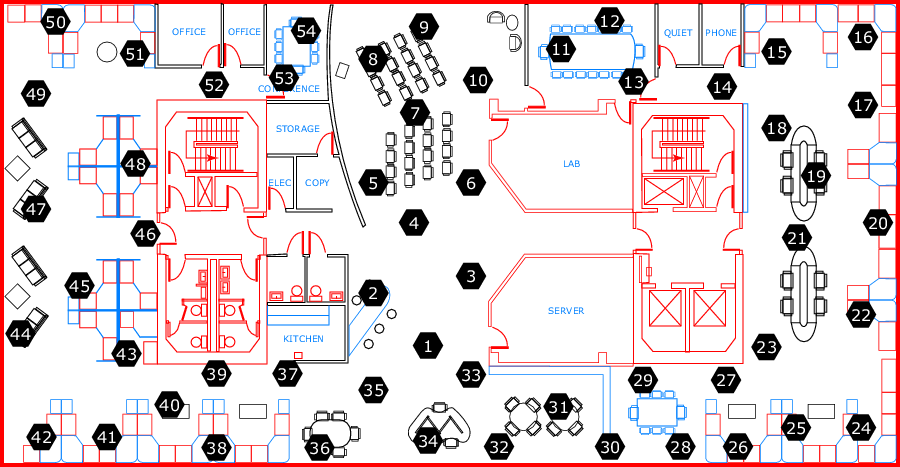
\includegraphics[scale=.25]{Figs/ibrl_wsn.png}
\caption{A map of sensors' location. (Source: \cite{Buonadonna2005})}
\label{fig:sensor_map}
\end{figure}

In this paper we consider the IBRL data set obtained from $5$ close nodes, $1, 2, 33, 35, 37$. Also, only two features, namely temperature and humidity, are taken into account. The data during the first $10$ days period on March 2004 will be used as the training set. This training set contains more than $82000$ samples. 

In order to evaluate performance of the proposed method, we also use a testing set in some concrete time intervals. Since the original data did not contain any labels as to which data is normal and anomalous, we visually identify and label them as normal and anomalous. This data set contains about $10000$ normal and $4000$ anomalous samples.

\subsection{Numerical results}

First, we use the Matlab's routine \emph{consolidator($\cdot$)}\footnote{https://mathworks.com/matlabcentral/fileexchange/8354-consolidator} to reduce the cardinality of training set into only $55421$ samples.

Fig.~\ref{fig:lof} shows the normal and anomalous sets produced by using  LOF method whereas $k = 50 \text{, } b = 1 \%$, $54866$ normal and $555$ anomalous samples are obtained. Notes however that this raw detection is likely wrong but it is helpful for computing the g-mean metric.  
\begin{figure}[H]
\centering
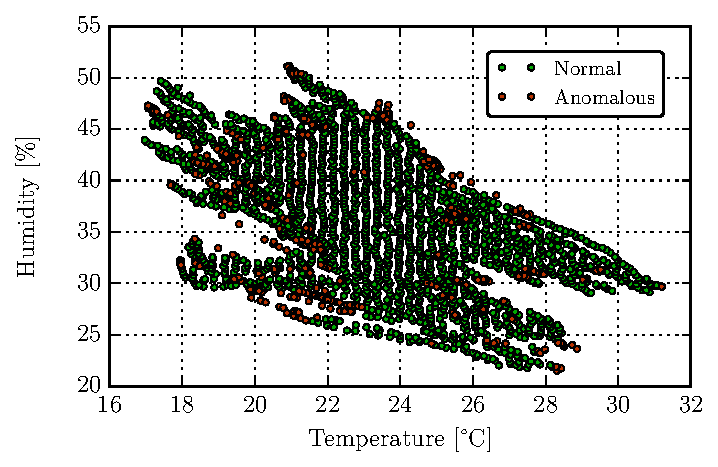
\includegraphics[scale=.6]{Figs/lof.pdf}
\caption{LOF detection result with $k = 50$ and $b = 1 \%$.}
\label{fig:lof}
\end{figure}

These samples will be hereafter used for training the SVDD given a grid of $\delta$'s values as:
\begin{align}
\delta \in \{ 0.001, 0.005, 0.01, 0.02, 0.03, 0.05, 0.1 \}
\end{align}
For details, solutions of the kernelized dual optimisation \eqref{eq:svm_dual_kernel} are obtained using the IBM ILOG CPLEX solver while optimal hyperparameters $(C,\sigma)$ are given by means of Bayesian optimization using the NLopt package \cite{nlopt}. Fig.~\ref{fig:domain_boundary} illustrates obtained decision boundaries. It is evident that with $0.01 \le \delta \le 0.05$, the distribution of considered data can be well estimated. 
\begin{figure}[H]
\centering
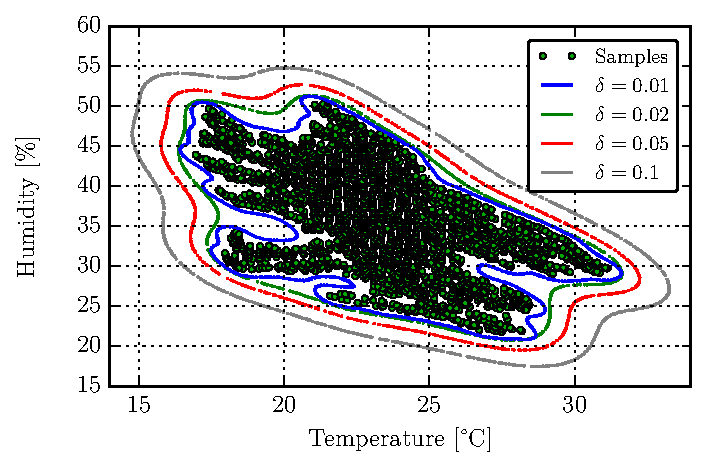
\includegraphics[scale=.6]{Figs/data_description.pdf}
\caption{Discrimination boundaries with some $\delta$'s values. The samples are normal data obtained from local outlier factor detection. The distribution of IBRL data is well estimated with sufficiently large threshold $\delta$. Also, low values of threshold $\delta$ may lead to sensitivity of the anomaly detection algorithm.}
\label{fig:domain_boundary}
\end{figure}

Table 1 presents the DR and FPR obtained. Although with $\delta \ge 0.02$, these performance indices are surpringly satisfactory, these results might be unreliable as well as conservative. Since the FPR is generally assumed to be about $5 \%$, the choices of $\delta=0.01$ or $0.02$ may be appropriate. 
\begin{table}[H]
\begin{tabular}{lccccccc}
\toprule
$\delta$ & 0.001 & 0.005 & 0.01 & 0.02 & 0.03 & 0.05 & 0.1 \\\midrule[\lightrulewidth]
DR [\%] & 100 & 100 & 100 & 100 & 100 & 100 & 100 \\
\emph{FPR} [\%] & 29.61 & 5.66 & 3.45 & 0 & 0 & 0 &0 \\\bottomrule
\end{tabular}
\caption{DR and FPR versus $\delta$.}
\label{table:delta_eval}
\end{table}

Fig.~\ref{fig:time_valid} depicts detection result on considered nodes over time with $\delta=0.02$, $C=0.5025$ and $\sigma=0.5039$. While perfect DR is admitted as in the Table 1, one can observe some false alarms which is acceptable.
\begin{figure*}
\centering
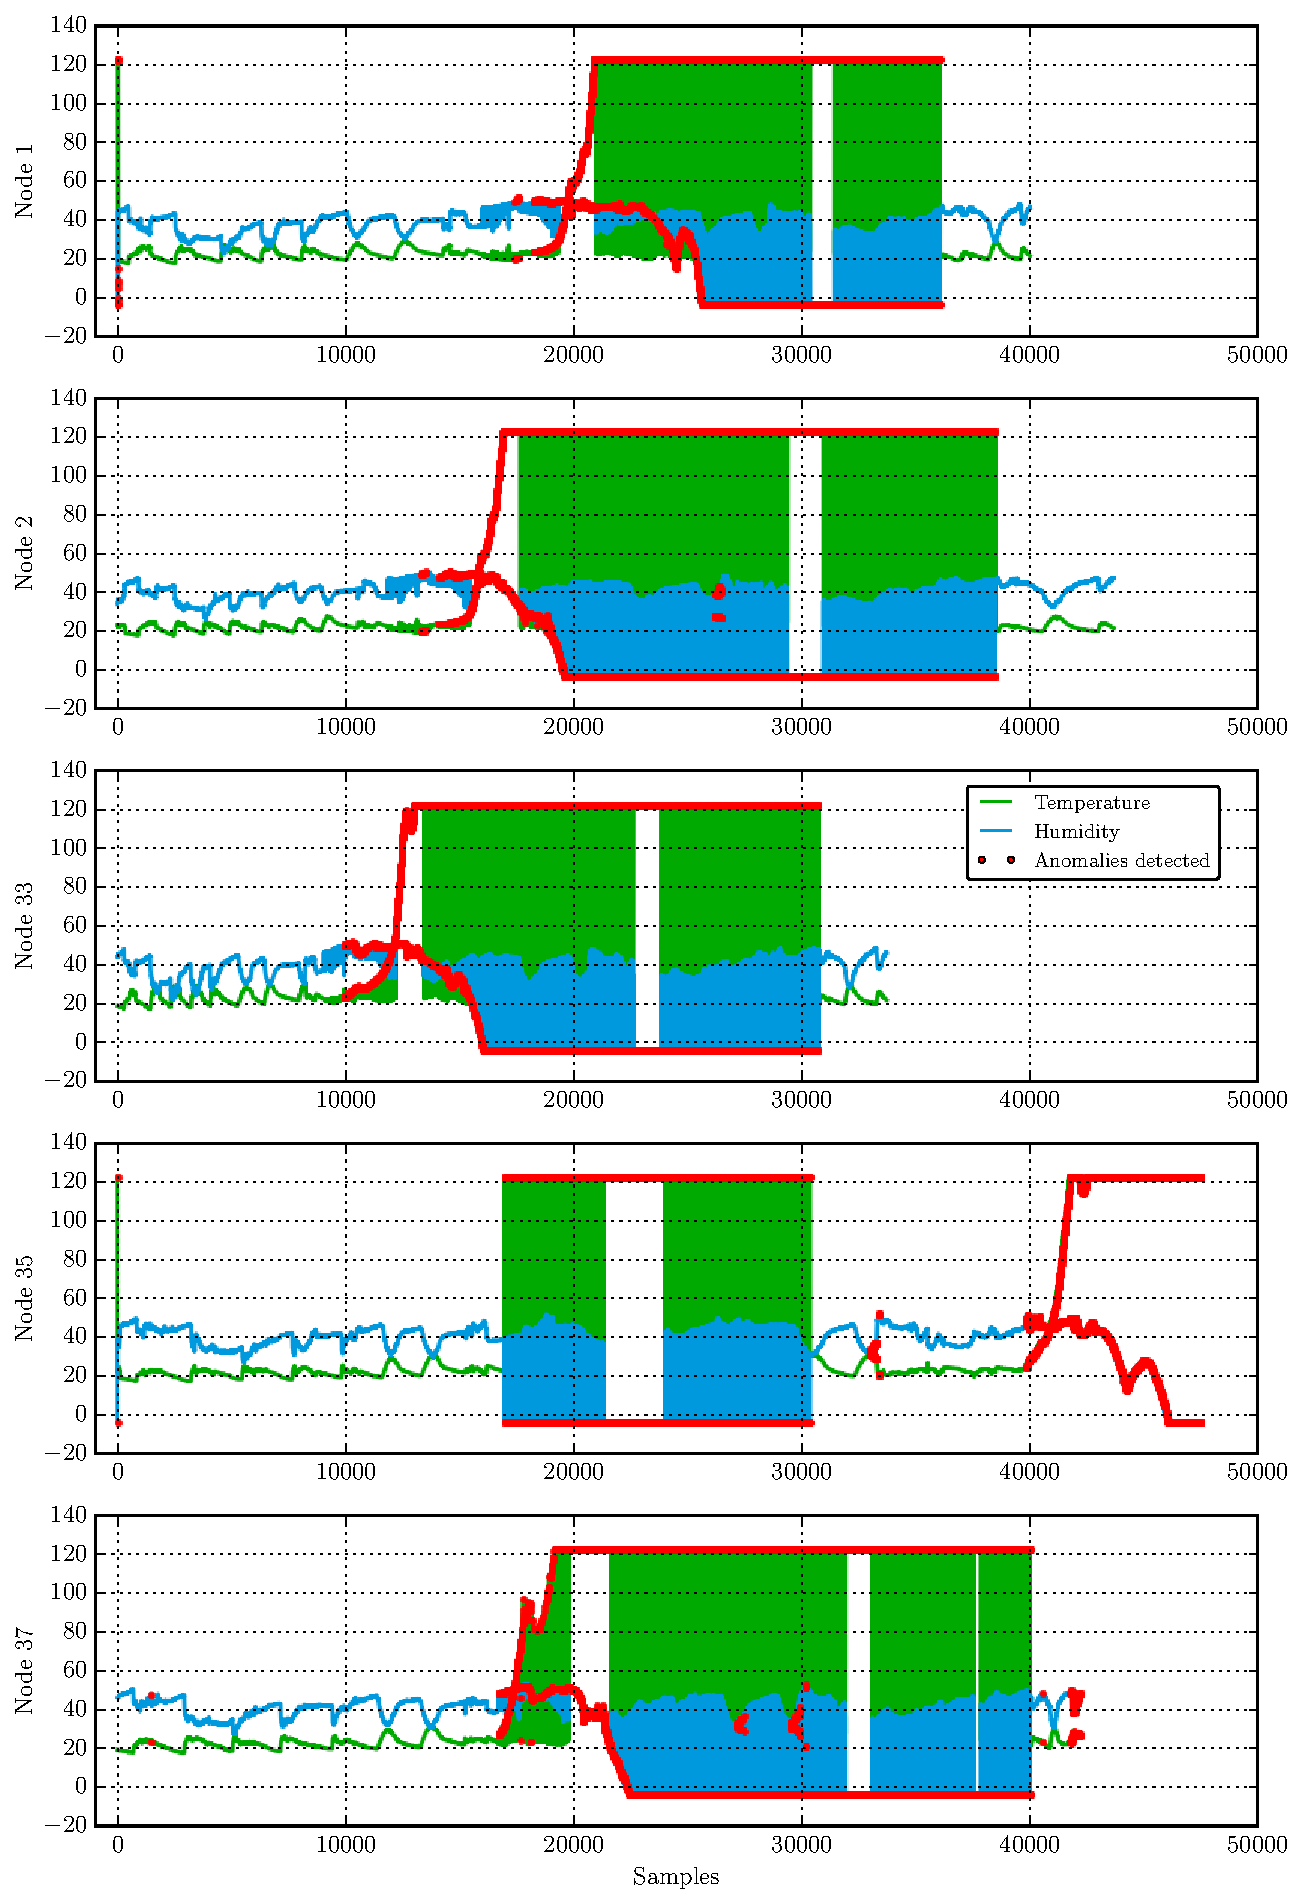
\includegraphics[scale=.7]{Figs/time_validation.pdf}
\caption{Anomaly detection validation upon whole IBRL data set on $5$ nodes. All apparent anomalies, i.e. temperature and humidity measurements that are too high or too low, are detected. Although nodes $35$ and $37$ exhibit several false alarms, such a fault detection is unavoidable and acceptable in practice.}
\label{fig:time_valid}
\end{figure*}

\section{Concluding remarks}\label{sec:concluding}

We presented a novel anomaly detection approach using SVDD in WSNs. Unlike the existing techniques which are all based on the RBF kernels, we developed an even more robust approach by incorporating the Mahalanobis kernels. Numerical result shown that the proposed approach achieved a high-level of detection accuracy and a low false alarm rate with appropriate  discriminative threshold.  

In the future, we would like to address the anomaly detection problem using autoencoder and control charts, targeting on time series data with uncertainties. We also focus on the detection ability of our proposed approach for large stream data.

\bibliographystyle{IEEEtran}
\bibliography{wsnbib,svmbib,ocsvmbib,ibrlbib,miscbib}

\end{document}


